\documentclass[twoside]{book}

% Packages required by doxygen
\usepackage{fixltx2e}
\usepackage{calc}
\usepackage{doxygen}
\usepackage[export]{adjustbox} % also loads graphicx
\usepackage{graphicx}
\usepackage[utf8]{inputenc}
\usepackage{makeidx}
\usepackage{multicol}
\usepackage{multirow}
\PassOptionsToPackage{warn}{textcomp}
\usepackage{textcomp}
\usepackage[nointegrals]{wasysym}
\usepackage[table]{xcolor}

% NLS support packages
Portuguese
% Font selection
\usepackage[T1]{fontenc}
\usepackage[scaled=.90]{helvet}
\usepackage{courier}
\usepackage{amssymb}
\usepackage{sectsty}
\renewcommand{\familydefault}{\sfdefault}
\allsectionsfont{%
  \fontseries{bc}\selectfont%
  \color{darkgray}%
}
\renewcommand{\DoxyLabelFont}{%
  \fontseries{bc}\selectfont%
  \color{darkgray}%
}
\newcommand{\+}{\discretionary{\mbox{\scriptsize$\hookleftarrow$}}{}{}}

% Page & text layout
\usepackage{geometry}
\geometry{%
  a4paper,%
  top=2.5cm,%
  bottom=2.5cm,%
  left=2.5cm,%
  right=2.5cm%
}
\tolerance=750
\hfuzz=15pt
\hbadness=750
\setlength{\emergencystretch}{15pt}
\setlength{\parindent}{0cm}
\setlength{\parskip}{3ex plus 2ex minus 2ex}
\makeatletter
\renewcommand{\paragraph}{%
  \@startsection{paragraph}{4}{0ex}{-1.0ex}{1.0ex}{%
    \normalfont\normalsize\bfseries\SS@parafont%
  }%
}
\renewcommand{\subparagraph}{%
  \@startsection{subparagraph}{5}{0ex}{-1.0ex}{1.0ex}{%
    \normalfont\normalsize\bfseries\SS@subparafont%
  }%
}
\makeatother

% Headers & footers
\usepackage{fancyhdr}
\pagestyle{fancyplain}
\fancyhead[LE]{\fancyplain{}{\bfseries\thepage}}
\fancyhead[CE]{\fancyplain{}{}}
\fancyhead[RE]{\fancyplain{}{\bfseries\leftmark}}
\fancyhead[LO]{\fancyplain{}{\bfseries\rightmark}}
\fancyhead[CO]{\fancyplain{}{}}
\fancyhead[RO]{\fancyplain{}{\bfseries\thepage}}
\fancyfoot[LE]{\fancyplain{}{}}
\fancyfoot[CE]{\fancyplain{}{}}
\fancyfoot[RE]{\fancyplain{}{\bfseries\scriptsize Gerado por Doxygen }}
\fancyfoot[LO]{\fancyplain{}{\bfseries\scriptsize Gerado por Doxygen }}
\fancyfoot[CO]{\fancyplain{}{}}
\fancyfoot[RO]{\fancyplain{}{}}
\renewcommand{\footrulewidth}{0.4pt}
\renewcommand{\chaptermark}[1]{%
  \markboth{#1}{}%
}
\renewcommand{\sectionmark}[1]{%
  \markright{\thesection\ #1}%
}

% Indices & bibliography
\usepackage{natbib}
\usepackage[titles]{tocloft}
\setcounter{tocdepth}{3}
\setcounter{secnumdepth}{5}
\makeindex

% Hyperlinks (required, but should be loaded last)
\usepackage{ifpdf}
\ifpdf
  \usepackage[pdftex,pagebackref=true]{hyperref}
\else
  \usepackage[ps2pdf,pagebackref=true]{hyperref}
\fi
\hypersetup{%
  colorlinks=true,%
  linkcolor=blue,%
  citecolor=blue,%
  unicode%
}

% Custom commands
\newcommand{\clearemptydoublepage}{%
  \newpage{\pagestyle{empty}\cleardoublepage}%
}

\usepackage{caption}
\captionsetup{labelsep=space,justification=centering,font={bf},singlelinecheck=off,skip=4pt,position=top}

%===== C O N T E N T S =====

\begin{document}

% Titlepage & ToC
\hypersetup{pageanchor=false,
             bookmarksnumbered=true,
             pdfencoding=unicode
            }
\pagenumbering{alph}
\begin{titlepage}
\vspace*{7cm}
\begin{center}%
{\Large Tratamento de Polígonos \\[1ex]\large 1.\+0.\+0.\+0 }\\
\vspace*{1cm}
{\large Gerado por Doxygen 1.8.13}\\
\end{center}
\end{titlepage}
\clearemptydoublepage
\pagenumbering{roman}
\tableofcontents
\clearemptydoublepage
\pagenumbering{arabic}
\hypersetup{pageanchor=true}

%--- Begin generated contents ---
\chapter{D\+C\+A1202\+\_\+\+Tratamento\+\_\+de\+\_\+poligonos}
\label{md__r_e_a_d_m_e}
\Hypertarget{md__r_e_a_d_m_e}
Primeiro projeto da segunda unidade da disciplina de Programação Avançada (D\+C\+A1202)

Instruções\+: (disponível em\+: \href{http://agostinhobritojr.github.io/cursos/progav/projetoscpp.html}{\tt http\+://agostinhobritojr.\+github.\+io/cursos/progav/projetoscpp.\+html})


\begin{DoxyEnumerate}
\item Projeto 1 -\/ Tratamento de polígonos Seu projeto deverá ser capaz de armazenar e realizar operações com polígonos formados por conjuntos de pontos em duas dimensões.
\end{DoxyEnumerate}

Deve ser previsto no projeto a criação de três classes\+:

\hyperlink{class_ponto}{Ponto}

\hyperlink{class_poligono}{Poligono}

\hyperlink{class_retangulo}{Retangulo}

1.\+1. Etapa 1 -\/ Criação da classe \hyperlink{class_ponto}{Ponto} Crie uma classe denominada Point para representar pontos no espaço bidimensional. Na sua implementação, você deverá encapsular duas variáveis x e y do tipo float para guardar a posição do ponto. Apenas as funções da classe poderão ter acesso direto a essas variávies, de modo que os clientes da classe somente poderão modificá-\/las usando métodos específicos que você definir. Implemente, na sua classe, métodos que realizem as seguintes operações\+:

Função Descrição set\+X(float) Define o valor da coordenada x do ponto. set\+Y(float) Define o valor da coordenada y do ponto. set\+X\+Y(float,float) Define, em uma mesma função, os valores da coordenadas x e y do ponto. float get\+X() Recupera o valor da coordenada x do ponto. float get\+Y() Recupera o valor da coordenada y do ponto. add(\+Point p1) Adiciona as coordenadas (x,y)(x,y) do ponto com as coordenadas de um ponto P1(x1,y1)P1(x1,y1) fornecido, armazenando o resultado (x+x1,y+y1)(x+x1,y+y1) nas coordenadas de um novo ponto, que deverá ser retornado para o cliente da classe. sub(\+Point p1) Subtrai as coordenadas (x,y)(x,y) do ponto com as coordenadas de um ponto P1(x1,y1)P1(x1,y1) fornecido, armazenando o resultado (x−x1,y−y1)(x-\/x1,y-\/y1) nas coordenadas de um novo ponto, que deverá ser retornado para o cliente da classe. norma() Calcula a distância do ponto para a origem do sistema de coordenadas. translada(float a, float b) Translada o ponto (x,y)(x,y) de (+a,+b)(+a,+b), de modo que, após a execução do método, as coordenadas do ponto serão (x+a,y+b)(x+a,y+b). imprime() Imprime o ponto na forma (xpos, ypos). 1.\+2. Etapa 2 -\/ Criação da classe \hyperlink{class_poligono}{Poligono} Defina uma classe chamada \hyperlink{class_poligono}{Poligono} para representar polígonos convexos. Assuma que o tamanho dos polígonos será limitado a 100 vértices. Utilize a classe Point que você definiu na etapa anterior para guardar informações com as posições dos NN vértices do polígono. Sua classe deverá prever as seguintes funcionalidades\+:

Inserir vértice no polígono. Assuma que os vértices deverão ser inseridos conforme a sequência (anti-\/horária) em que figuram ao redor do polígono. As arestas do polígono serão então compostas pelos segmentos (x0,y0)→(x1,y1)(x0,y0)→(x1,y1), (x1,y1)→(x2,y2)(x1,y1)→(x2,y2) etc., com exceção da última aresta, que será formada pelo segmento (x\+N−1,y\+N−1)→(x0,y0)(x\+N−1,y\+N−1)→(x0,y0).

Recuperar a quantidade de vértices que foram inseridos no polígono

Calcular a área do polígono. Procure na Internet a fundamentação matemática necessária para implementar essa funcionalidade.

Transladar o polígono para (+a,+b)(+a,+b) usando uma função translada(float a, float b).

Rotacionar o polígono de θθ graus no sentido anti-\/horário em torno de um ponto (x0,y0)(x0,y0) fornecido pelo usuário.

Imprimir o polígono armazenado da forma (x0,y0)→(x1,y1)→(x2,y2)→…​

1.\+3. Etapa 3 -\/ Criação da classe \hyperlink{class_retangulo}{Retangulo} Utilizando a implementação da classe \hyperlink{class_poligono}{Poligono} desenvolvida na etapa anterior, crie uma subclasse \hyperlink{class_retangulo}{Retangulo} derivada da superclasse \hyperlink{class_poligono}{Poligono}. O construtor da nova classe deverá ser da forma \hyperlink{class_retangulo}{Retangulo(float x, float y, float largura, float altura)}, denotando a posição (x,y)(x,y) do retângulo no espaço (coordenadas do canto superior esquerdo) e suas dimensões -\/ altura e largura. Realize com esta classe as seguintes tarefas\+:

Assegure-\/se de que o construtor da classe utiliza os métodos da superclasse para armazenar a estrutura interna do retângulo.

1.\+4. Etapa 4 -\/ Teste das classes criadas Crie um pequeno exemplo para testar sua implementação da classe \hyperlink{class_retangulo}{Retangulo}.

No exemplo, defina um novo retângulo na posição (x,y)=(0,0)(x,y)=(0,0), com altura e largura iguais a 3 e 4, respectivamente.

Imprima a estrutura poligonal gerada para o retângulo.

Calcule a sua área usando a função já implementada na classe \hyperlink{class_poligono}{Poligono} e mostre o resultado.

Mude a posição do retângulo usando a função translada(float,float) para (x,y)=(−3,4)(x,y)=(-\/3,4) e recalcule a área do retângulo. Compare-\/a com a área calculada antes da transformação geométrica.

Rotacione o Retângulo de +30o+30o em relação ao seu centro de massa e recalcule a sua área. Compare-\/a com a área calculada antes da transformação geométrica. 
\chapter{Índice da hierarquia}
\section{Hierarquia de classes}
Esta lista de heranças está organizada, dentro do possível, por ordem alfabética\+:\begin{DoxyCompactList}
\item \contentsline{section}{Point}{\pageref{class_point}}{}
\begin{DoxyCompactList}
\item \contentsline{section}{Polygon}{\pageref{class_polygon}}{}
\end{DoxyCompactList}
\item \contentsline{section}{Rectangle}{\pageref{class_rectangle}}{}
\end{DoxyCompactList}

\chapter{Índice dos componentes}
\section{Lista de componentes}
Lista de classes, estruturas, uniões e interfaces com uma breve descrição\+:\begin{DoxyCompactList}
\item\contentsline{section}{\hyperlink{class_point}{Point} }{\pageref{class_point}}{}
\item\contentsline{section}{\hyperlink{class_polygon}{Polygon} }{\pageref{class_polygon}}{}
\item\contentsline{section}{\hyperlink{class_rectangle}{Rectangle} }{\pageref{class_rectangle}}{}
\end{DoxyCompactList}

\chapter{Documentação da classe}
\hypertarget{class_point}{}\section{Referência à classe Point}
\label{class_point}\index{Point@{Point}}
Diagrama de heranças da classe Point\begin{figure}[H]
\begin{center}
\leavevmode
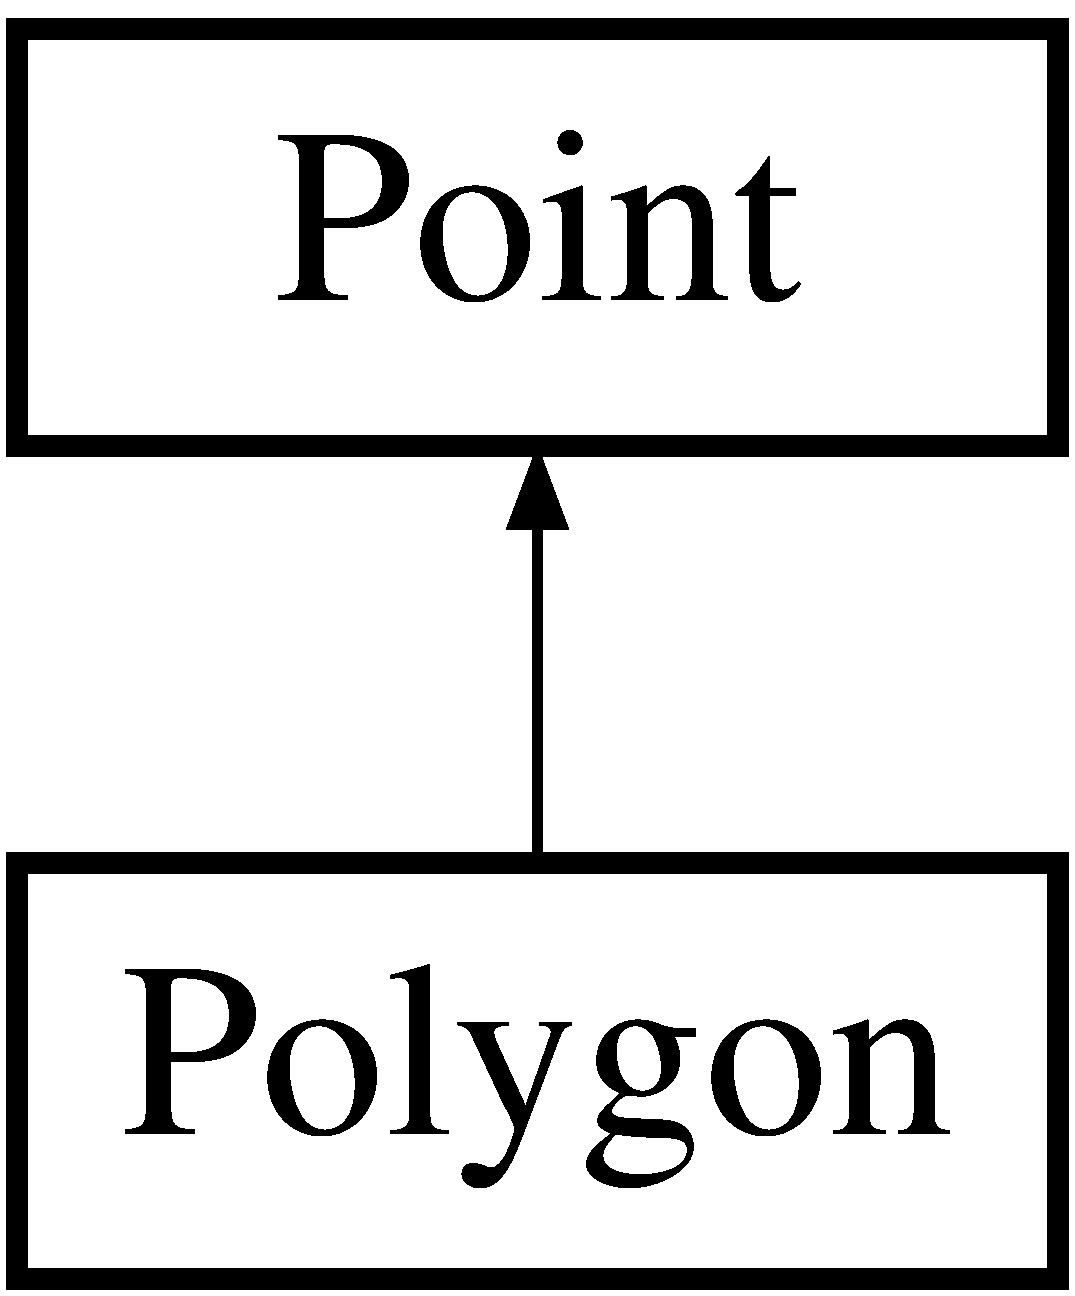
\includegraphics[height=2.000000cm]{class_point}
\end{center}
\end{figure}
\subsection*{Membros públicos}
\begin{DoxyCompactItemize}
\item 
\mbox{\Hypertarget{class_point_a71e14784800fdf014b1dad07042b6b58}\label{class_point_a71e14784800fdf014b1dad07042b6b58}} 
void {\bfseries setX} (float \+\_\+x=0)
\item 
\mbox{\Hypertarget{class_point_a1a662e77ed872c6528baa01ded1cfea6}\label{class_point_a1a662e77ed872c6528baa01ded1cfea6}} 
void {\bfseries setY} (float \+\_\+y=0)
\item 
\mbox{\Hypertarget{class_point_ab05bb91232ba62143456855b81db5ed0}\label{class_point_ab05bb91232ba62143456855b81db5ed0}} 
void {\bfseries set\+XY} (float \+\_\+x=0, float \+\_\+y=0)
\item 
\mbox{\Hypertarget{class_point_acc27466778cc87a662bba40268c4c0c8}\label{class_point_acc27466778cc87a662bba40268c4c0c8}} 
float {\bfseries getX} ()
\item 
\mbox{\Hypertarget{class_point_a3cccbca94719ddde353cce86ce0e2f64}\label{class_point_a3cccbca94719ddde353cce86ce0e2f64}} 
float {\bfseries getY} ()
\item 
\mbox{\Hypertarget{class_point_ad73d7e70a1d4ff675c98fdcc29bd3f49}\label{class_point_ad73d7e70a1d4ff675c98fdcc29bd3f49}} 
\hyperlink{class_point}{Point} {\bfseries operator+} (\hyperlink{class_point}{Point} p1)
\item 
\mbox{\Hypertarget{class_point_ab5658ed6bab41aa67a6f62536d782868}\label{class_point_ab5658ed6bab41aa67a6f62536d782868}} 
\hyperlink{class_point}{Point} {\bfseries operator-\/} (\hyperlink{class_point}{Point} p1)
\item 
\mbox{\Hypertarget{class_point_a4c302c05a75713df428361264b3eb1b3}\label{class_point_a4c302c05a75713df428361264b3eb1b3}} 
double {\bfseries norma} ()
\item 
\mbox{\Hypertarget{class_point_a69851f251df64023a2661c56c6273e2f}\label{class_point_a69851f251df64023a2661c56c6273e2f}} 
void {\bfseries translada} (float a=0, float b=0)
\item 
\mbox{\Hypertarget{class_point_a1fb5c2501c27ab2cbc99d06c2a26a741}\label{class_point_a1fb5c2501c27ab2cbc99d06c2a26a741}} 
void {\bfseries imprime} ()
\end{DoxyCompactItemize}


A documentação para esta classe foi gerada a partir dos seguintes ficheiros\+:\begin{DoxyCompactItemize}
\item 
point.\+h\item 
point.\+cpp\end{DoxyCompactItemize}

\hypertarget{class_polygon}{}\section{Referência à classe Polygon}
\label{class_polygon}\index{Polygon@{Polygon}}
Diagrama de heranças da classe Polygon\begin{figure}[H]
\begin{center}
\leavevmode
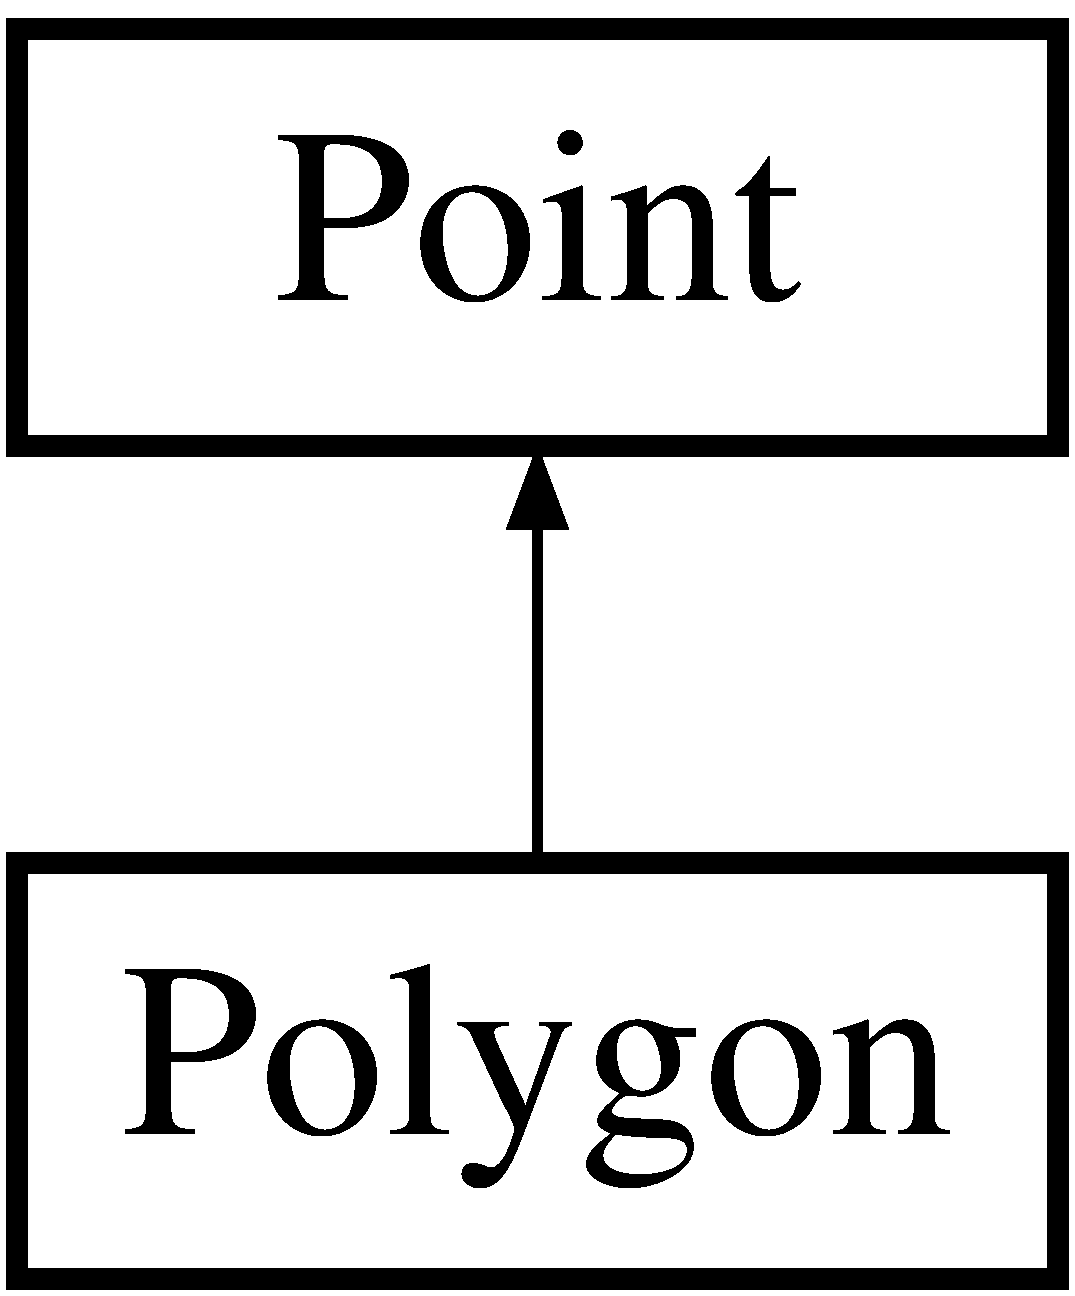
\includegraphics[height=2.000000cm]{class_polygon}
\end{center}
\end{figure}
\subsection*{Membros públicos}
\begin{DoxyCompactItemize}
\item 
\mbox{\Hypertarget{class_polygon_a1ef47b98e579dd5e53744980fb822ab2}\label{class_polygon_a1ef47b98e579dd5e53744980fb822ab2}} 
void {\bfseries add\+Vertex} (\hyperlink{class_point}{Point} \+\_\+vertex)
\item 
\mbox{\Hypertarget{class_polygon_aab9e9609b0ec0991f0be9099f4d48673}\label{class_polygon_aab9e9609b0ec0991f0be9099f4d48673}} 
int {\bfseries num\+Vertices} (\hyperlink{class_point}{Point} $\ast$v)
\item 
double \hyperlink{class_polygon_a1605b702a19992a4631aa1011092c0c1}{area} (\hyperlink{class_point}{Point} $\ast$vertices, int n\+Vert)
\begin{DoxyCompactList}\small\item\em Calcula a área do polígono usando as coordenadas de seus vértices. \end{DoxyCompactList}\item 
\mbox{\Hypertarget{class_polygon_a082ff056dc124290a464b0b718212d02}\label{class_polygon_a082ff056dc124290a464b0b718212d02}} 
void {\bfseries translada} (float a, float b)
\item 
\mbox{\Hypertarget{class_polygon_a7f7ef8b0f44d5d063989f777c6afdbe9}\label{class_polygon_a7f7ef8b0f44d5d063989f777c6afdbe9}} 
void {\bfseries rotate} (float theta)
\item 
\mbox{\Hypertarget{class_polygon_a60830487fc3c6b815aa577e9dd758b51}\label{class_polygon_a60830487fc3c6b815aa577e9dd758b51}} 
void {\bfseries print} ()
\end{DoxyCompactItemize}


\subsection{Documentação dos métodos}
\mbox{\Hypertarget{class_polygon_a1605b702a19992a4631aa1011092c0c1}\label{class_polygon_a1605b702a19992a4631aa1011092c0c1}} 
\index{Polygon@{Polygon}!area@{area}}
\index{area@{area}!Polygon@{Polygon}}
\subsubsection{\texorpdfstring{area()}{area()}}
{\footnotesize\ttfamily double Polygon\+::area (\begin{DoxyParamCaption}\item[{\hyperlink{class_point}{Point} $\ast$}]{vertices,  }\item[{int}]{n\+Vert }\end{DoxyParamCaption})}



Calcula a área do polígono usando as coordenadas de seus vértices. 

O algoritmo do cálculo da área funciona como se as coordenadas dos vértices tivessem sido organizados em uma tabela, repetindo-\/se as primeiras coordenadas na última linha, e em-\/seguida tivessem sido multiplicadas e somadas todas as diagonais principais , operação feita em 
\begin{DoxyParams}{Parâmetros}
{\em diag\+Princ} & \\
\hline
\end{DoxyParams}


A documentação para esta classe foi gerada a partir dos seguintes ficheiros\+:\begin{DoxyCompactItemize}
\item 
polygon.\+h\item 
polygon.\+cpp\end{DoxyCompactItemize}

\hypertarget{class_rectangle}{}\section{Referência à classe Rectangle}
\label{class_rectangle}\index{Rectangle@{Rectangle}}


A documentação para esta classe foi gerada a partir do seguinte ficheiro\+:\begin{DoxyCompactItemize}
\item 
rectangle.\+h\end{DoxyCompactItemize}

%--- End generated contents ---

% Index
\backmatter
\newpage
\phantomsection
\clearemptydoublepage
\addcontentsline{toc}{chapter}{Índice}
\printindex

\end{document}
